\documentclass[pdftex,a4paper,12pt,twocolumn,fleqn,captions=tableheading]{scrartcl}

\usepackage[british]{babel}
\usepackage[utf8]{inputenc}
\usepackage[T1]{fontenc}
\usepackage{graphicx}
\usepackage{booktabs}
\usepackage{caption}
\usepackage{subcaption}
\usepackage{lmodern}
\usepackage{microtype}
\usepackage{textcomp}
\usepackage{amssymb}
\usepackage{epstopdf}
\usepackage{capt-of}
\usepackage{amsmath}
\usepackage{float}
\usepackage{xfrac}
\usepackage{dblfloatfix}
\usepackage{url}
\usepackage[squaren,Gray]{SIunits}
\usepackage{commath}
\usepackage{listings}
% \usepackage{siunitx}

\addtokomafont{caption}{\small}
\setkomafont{captionlabel}{\sffamily\bfseries}

\usepackage[nottoc]{tocbibind}

% page layout
\usepackage[a4paper,onecolumn]{geometry}
\geometry{hmargin=60pt,top=60pt,bottom=80pt}
% \geometry{onecolumn,columnsep=20pt}
\geometry{head=10pt,headsep=20pt,foot=35pt}

% header and footer
\usepackage{fancyhdr}
\setlength{\headheight}{15pt}
\pagestyle{fancy}
%\fancyheadoffset{9pt}
%\fancyfootoffset{9pt}
\lhead{}	\chead{User manual IMU instruments with Iridium communications}	\rhead{}
\lfoot{}	\cfoot{J. Rabault \\ \thepage}	\rfoot{}
%\renewcommand{\headrulewidth}{0,1 mm}
\renewcommand{\footrulewidth}{\headrulewidth}

\begin{document}
% top matter
\title{Using the waves in ice IMU instruments with Iridium communications}
\author{J. Rabault
  }
\date{\today}

\maketitle

This is a short user manual for the IMU waves in ice instruments with Iridium communications. In all the following, I describe how the instruments are set up after assembly at UiO, but it should be roughly the same also if they are built in-house by another group. For more details about the instrument, see the detailed paper (Rabault et. al., Cold Region Science and Technology (2020), "An Open Source, Versatile, Affordable Waves in Ice Instrument for Remote Sensing in the Polar Regions"), available as a preprint at: ~\\

\url{https://www.researchgate.net/publication/330241626_An_Open_Source_Versatile_Affordable_Waves_in_Ice_Instrument_for_Remote_Sensing_in_the_Polar_Regions}.

\section{Introduction}

The instrument has a few main components:

\begin{itemize}
  \item Master PCB, including voltage regulator, SD card, GPS connected to its antenna, and some various small components, which are set up on top of an Arduino Mega.
  \item Iridium moden connected to its antenna.
  \item Raspberry Pi microcomputer.
  \item Solar panel and battery.
  \item Inertial Motion Unit (IMU, possibly hidden at the bottom of the box depending on the assembly).
\end{itemize}

All the components are visible on following pictures \ref{FromOutside} and \ref{FromInside}.

  \begin{figure}
  \begin{center}
  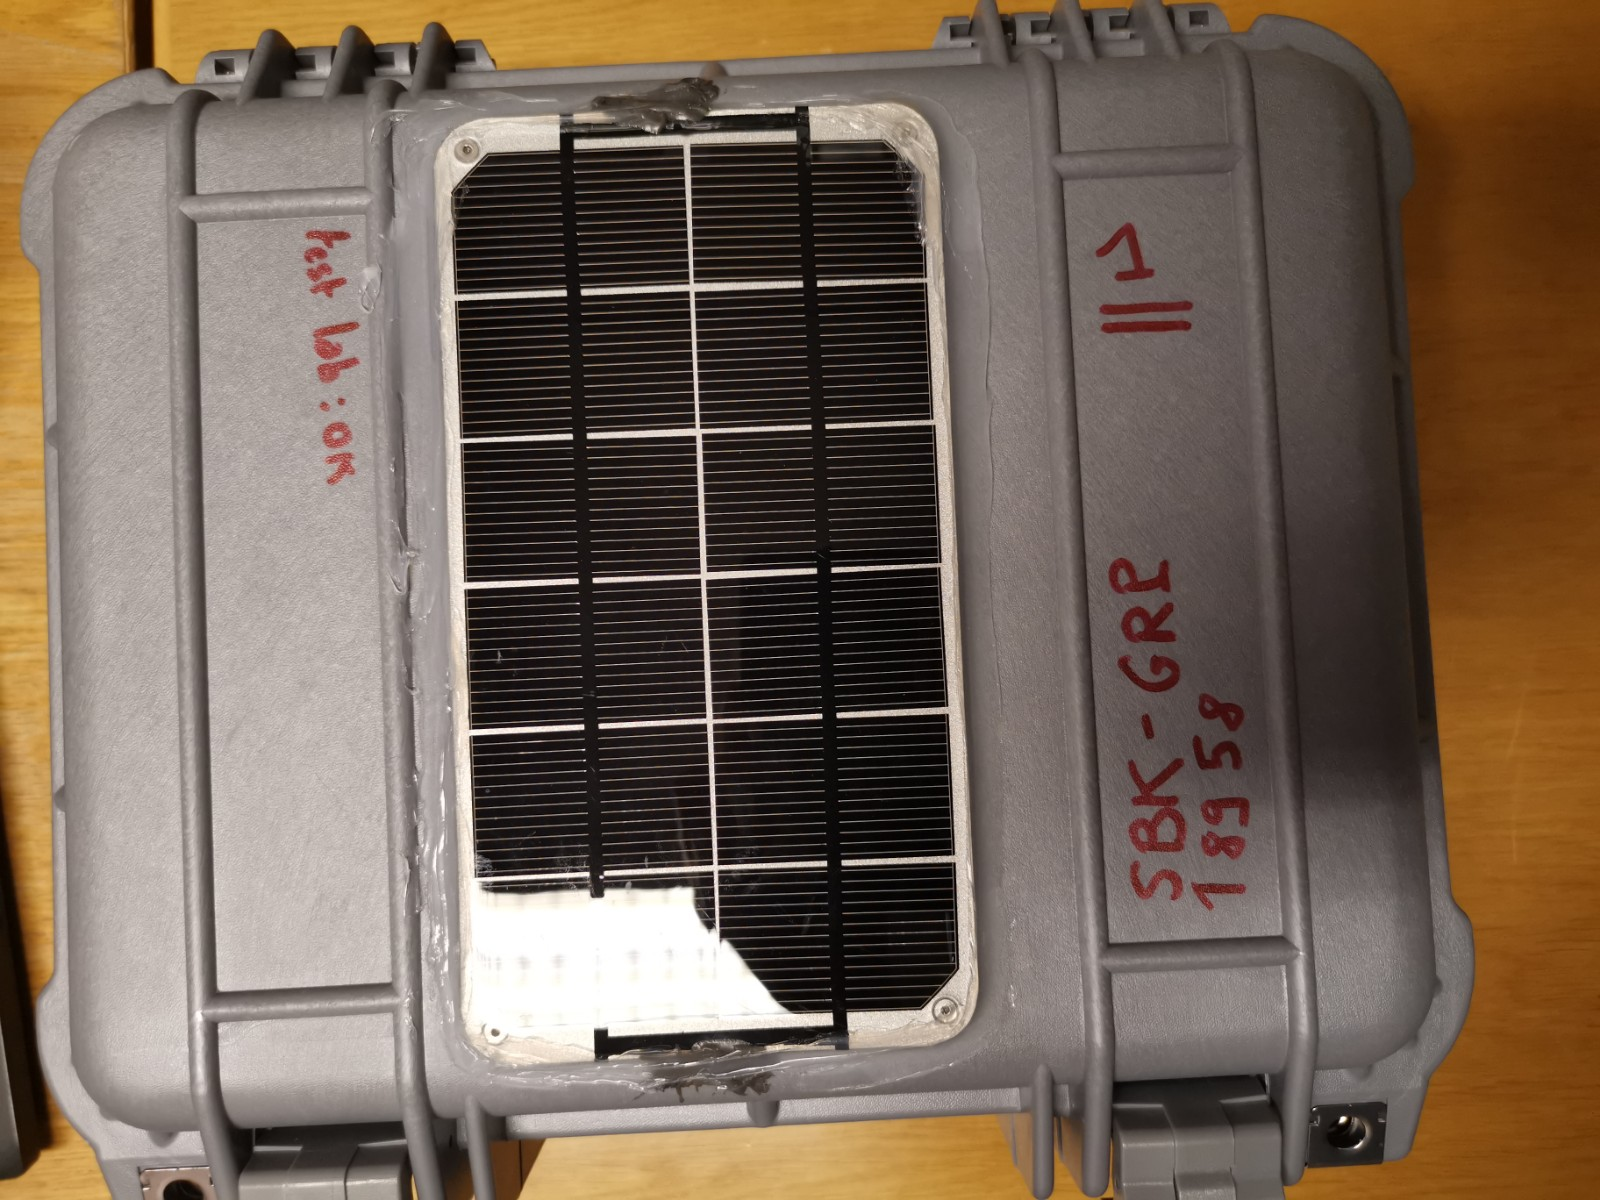
\includegraphics[width=.8\textwidth]{Figures/IMG_20200616_161755}
  \caption{\label{FromOutside} The instrument seen from the top, with solar panel, and a written copy of the Iridium modem reference number (here, SBK-GRP 18958). In addition, each instrument in a production series is given a number, here this is instrument number 1.}
  \end{center}
  \end{figure}


  \begin{figure}
  \begin{center}
  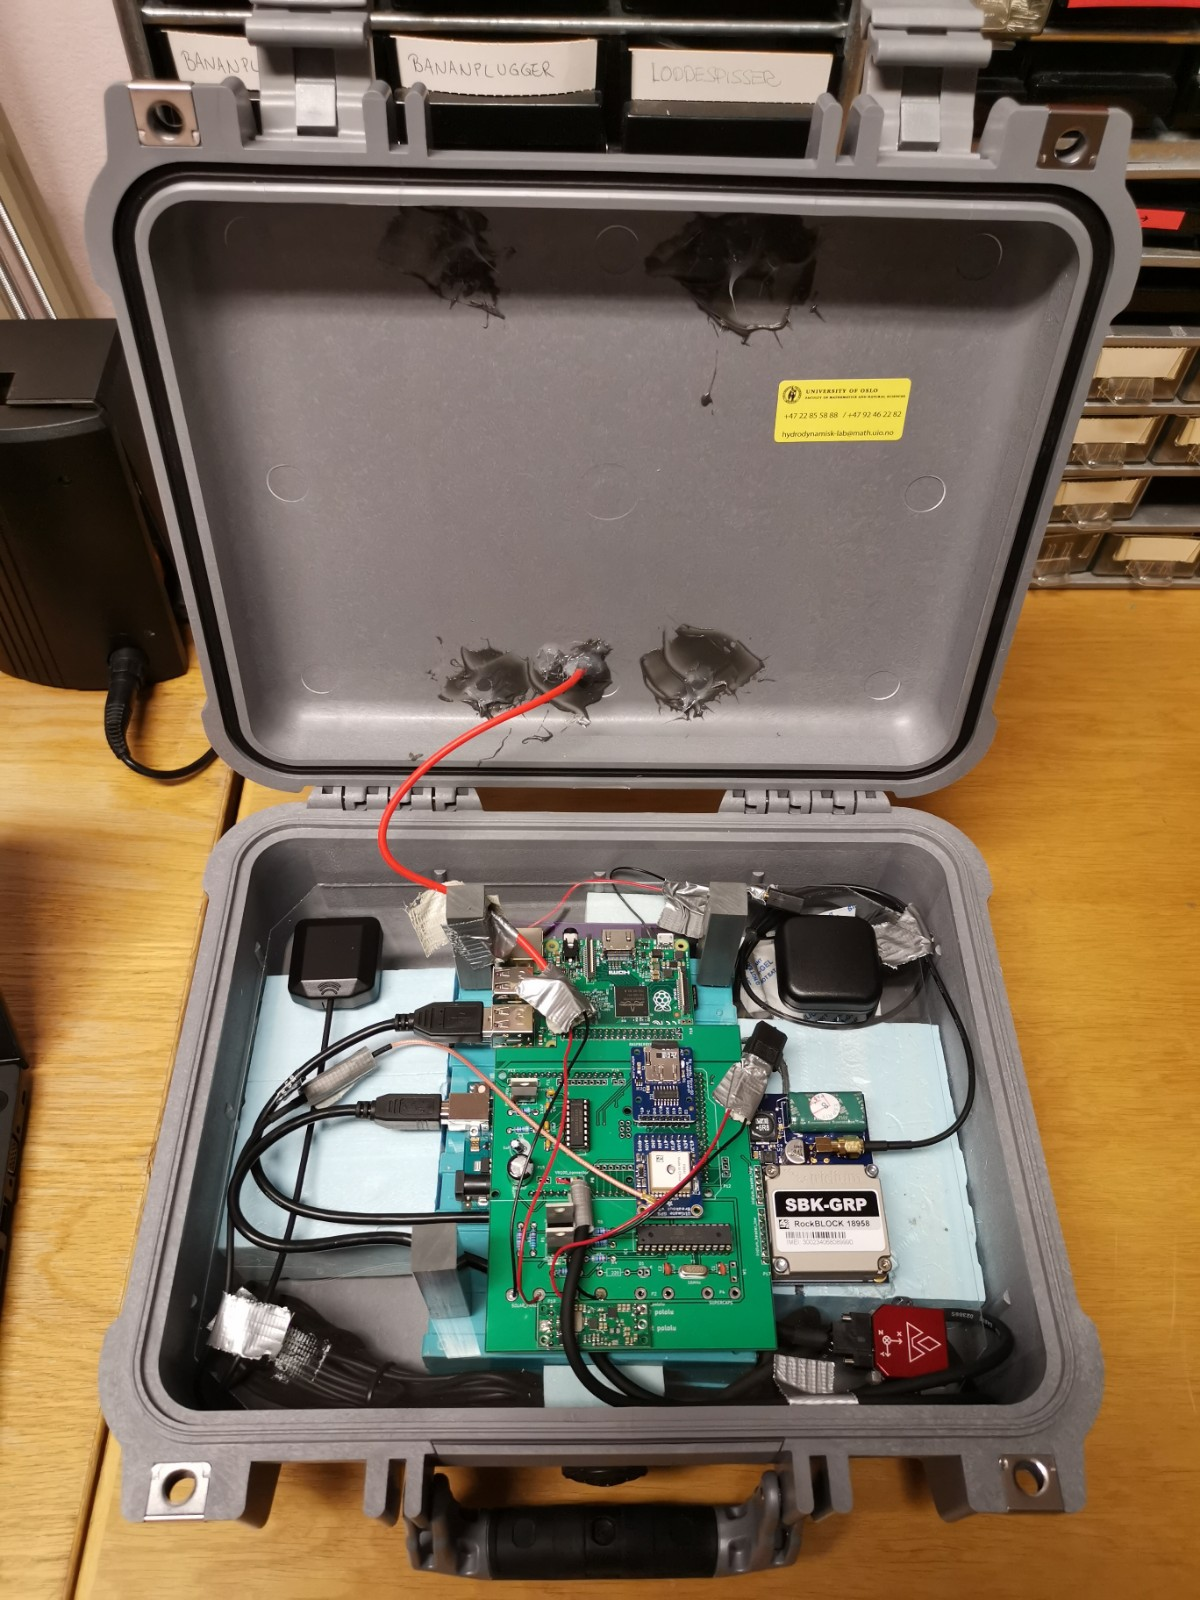
\includegraphics[width=.8\textwidth]{Figures/IMG_20200616_161730}
  \caption{\label{FromInside} The instrument seen inside. The different components are clearly visible: IMU (red component at the lower right), GPS antenna (upper left), Iridium antenna (upper right), main PCB on top of an Arduino Mega including SD card reader, GPS module, and small electronics, Iridium model (right), RaspberryPi microcontroller (top), USB cable linking Raspberry Pi and Arduino Mega, single cell battery at the bottom.}
  \end{center}
  \end{figure}

\section{Use}

Any instrument shipped has been fully tested at UiO and should work "out of the box". Instruments being shipped are powered off, and the only step necessary before use is to switch on the instruments (see following). In addition, you need to notify me (address: jean.rblt@gmail.com) before deployment so that I can start Iridium subscriptions for data transmission. If you want to receive a forwarding of the iridium data, send an additional email to the same address. ~\\

To deploy:

\begin{itemize}
  \item Open the instrument. Remember that electronics are very sensitive to static electricity discharges / sparks, so try to touch the PCBs / electronics as little as possible, and try to "dischare yourself" by touching a large metallic mass before opening the instrument. Try to only open the instrument either inside a vehicle, or outside when the conditions are good, so that no snow / water is introduced. Some dessicant bags are hidden at the bottom of the instrument, so it should be fairly resistant to a bit of humidity.
  \item Take a short visual inspection to make sure that the instrument was not damaged during transport: check visually that all cables are in place, and nothing looks broken (SD card inserted, USB cable in place, GPS antenna cable in place).
  \item Find the main power connectors. These should be the only 2 loose connectors present in the box. They may be taped inside the box to make sure that they do not "move around" during transport.
  \item Connect the 2 main power connectors. Make sure that you engage them fully all the way.
  \item At this stage, the GPS LED should start blinking. Depending on the number of sleep cycles left, either it will only blink for a few seconds before turning off (which means that the instrument goes into sleep mode until it should perform a measurement, this is normal), or it will continue blinking, and the SD card reader will start blinking too, in which case a measurement is starting (this is also normal behavior). If nothing blinks, you may consider the "troubleshooting" section. Note that the blinking may be quite low intensity and hard to see, especially outdoors.
  \item At this stage, the instrument is ready: close it and put it on the ice. Make sure that you do not pinch any cables when closing the top lid.
\end{itemize}

  \begin{figure}
  \begin{center}
  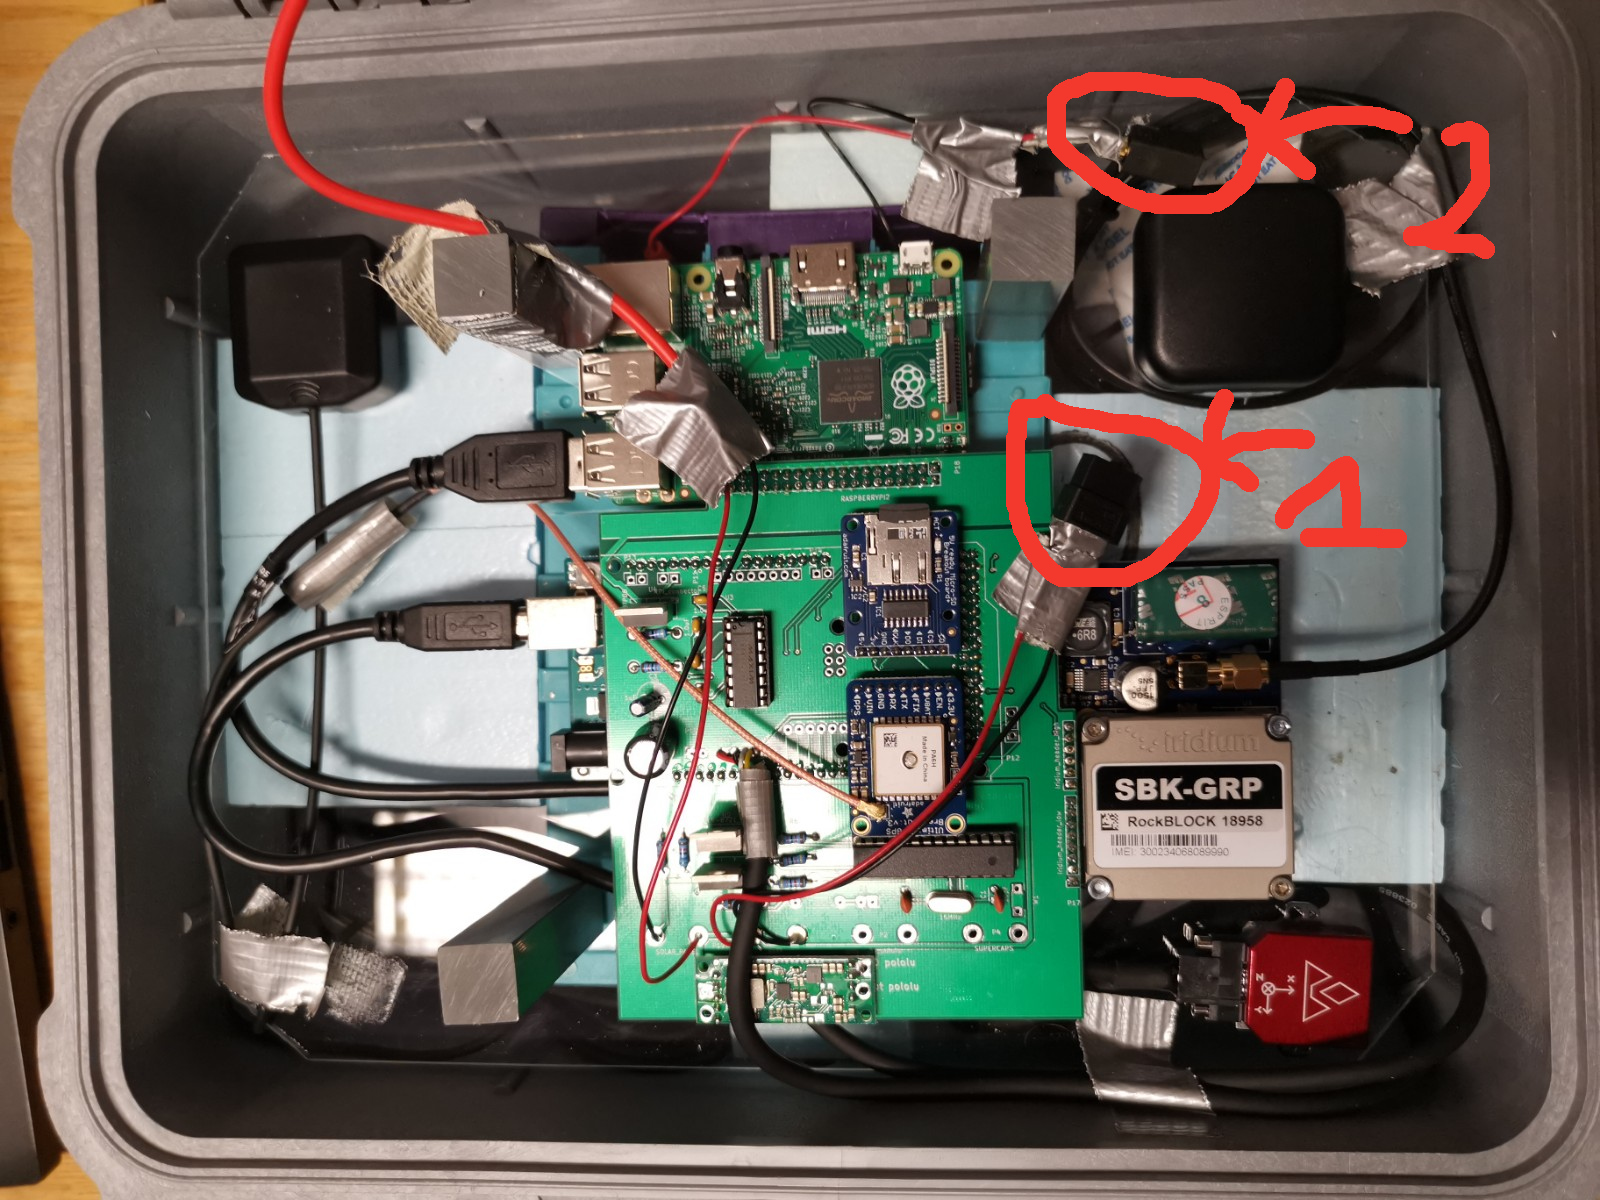
\includegraphics[width=.8\textwidth]{Figures/connectors}
  \caption{\label{Connector} The main power connectors are highlighted in red. Connect them fully and securely, and the instrument will start. Depending on the exact instrument, either the connector shown, or a slightly different connector model, may be used. Feel free to rip off the tape holding the connectors, this is only used to secure everything during transport. The connectors can only be inserted in the right polarisation direction.}
  \end{center}
  \end{figure}

Once this is done, the instrument will periodically transmit through Iridium its position and the wave information. The typical wake-up cycle is: 2.5 hours sleep, 0.5 hours logging, and sending of a message. ~\\

A few points about the instruments deployment:

\begin{itemize}
  \item Place the instrument directly on the ice. If there is a small layer of snow (up to half the height of the box), take away the snow, and put the instrument directly on the ice. Feel free to pack a bit of snow on all 4 sides of the instrument, to stabilize it, without covering it.
  \item The antenna immediately under the lid need a good vision of the sky in order to perform well, so it is important to try to deploy the instrument in a place where it is not too likely to get buried under snow.
  \item The box is water-proof and has buoyancy, however it does not float very well, especially without the addition of an external floater.
\end{itemize}

Try to not start / stop the instruments: just let them on for the full duration of the deployment if no problem is encountered. Do not try to disconnect any cables / remove SD cards or other. All relevant data are transmitted through Iridium anyways. If necessary, to stop the instruments:

\begin{itemize}
  \item Cover the solar panel with a dark, mate, opaque cover, and keey them covered the whole time of the procedure. If not, the solar panels will continue providing enough energy to keep the instruments on.
  \item Disconnect the main power connector. Secure both ends with a bit of tape.
  \item To make sure that all capacitors are emptied, and that all electronics is shut off rather than in compromized browned-out mode, use the provided cable to short the 2 "supercaps" pads, as visible in Fig. \ref{shorting}.
\end{itemize}

  \begin{figure}
  \begin{center}
  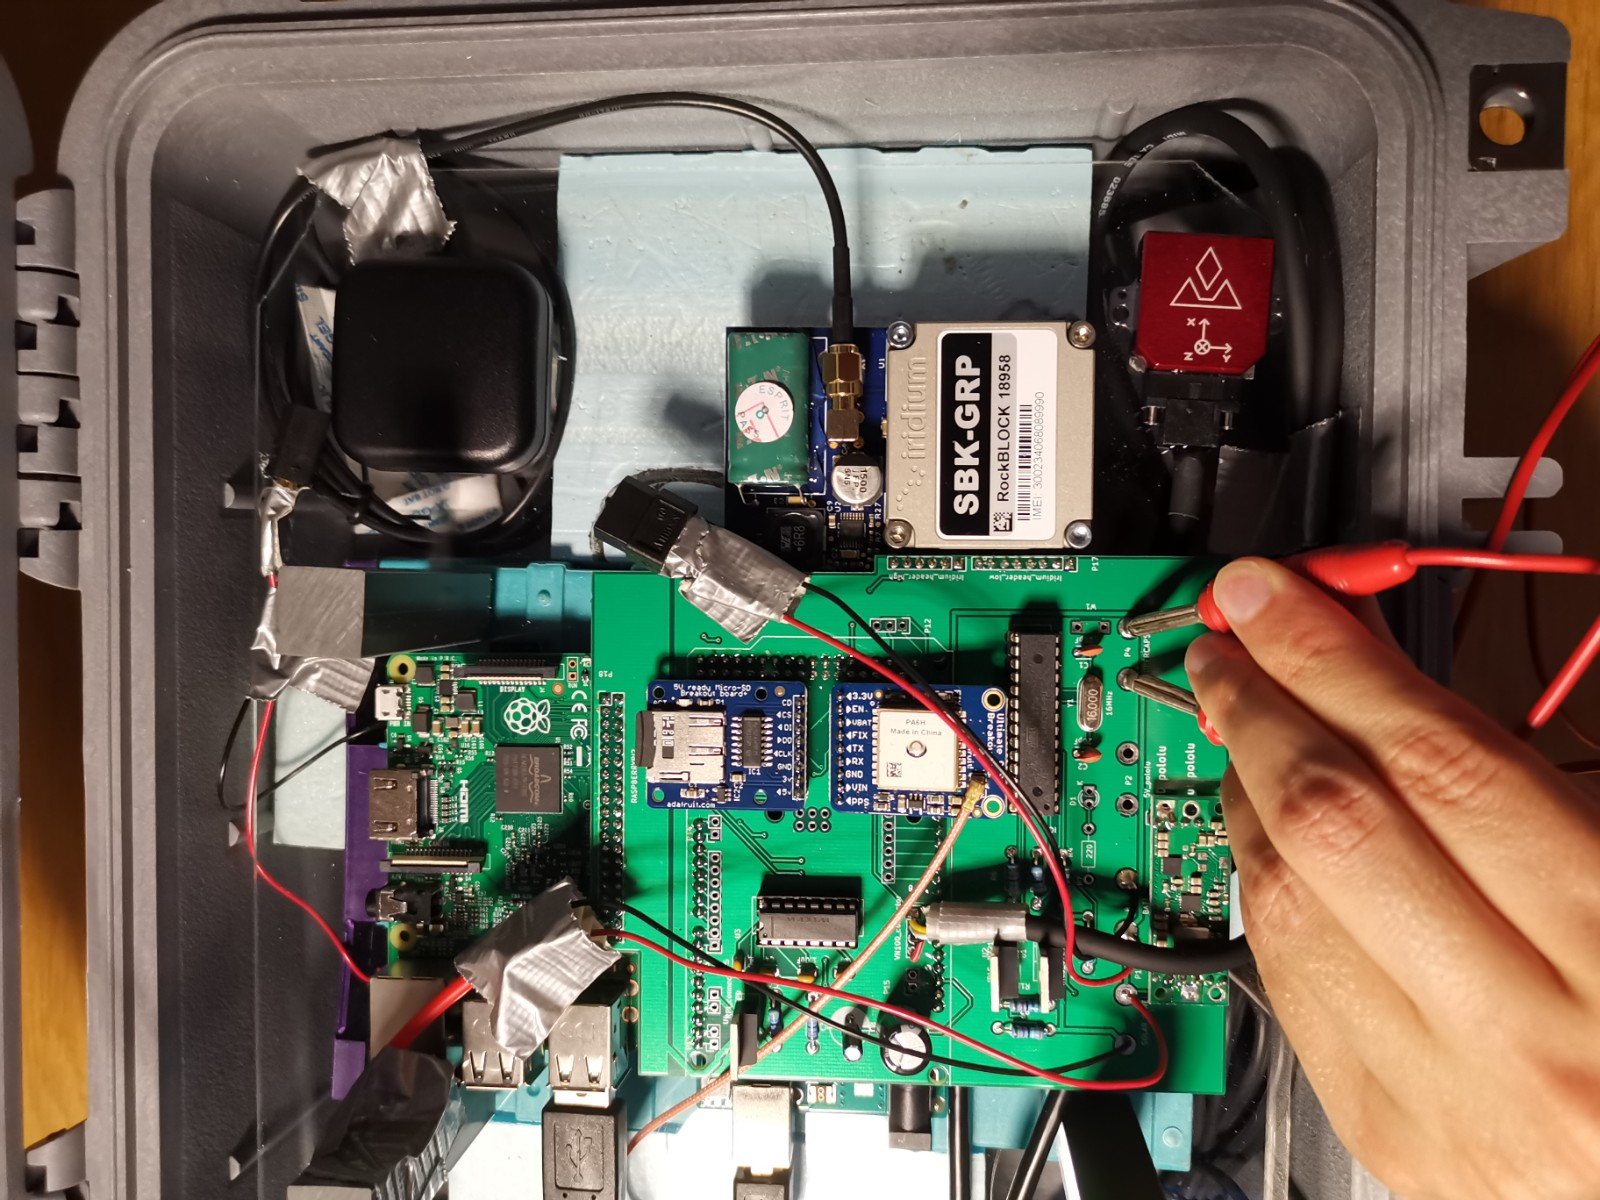
\includegraphics[width=.8\textwidth]{Figures/shorting}
  \caption{\label{shorting} shorting of the "supercaps" pins using the provided cable, in order to empty all capacitors and make sure that the electronics is not let in a browned-out state.}
  \end{center}
  \end{figure}

\section{Troubleshooting}

The design has been tested and operated without problems in several campaigns, both in the Arctic and the Antarctic.

The main possible sources of troubles include: 1) the instruments being covered by snow 2) the instruments being destroyed by polar bears 2) the instruments falling in the water / being crushed following ice breakup.

The instruments should have enough power through the solar panel to sustain continuous operation with around 8 to 10 hours of sun per day. The batteries included should allow operation without any solar input for at least 1 to 2 months depending on the frequency of data transmission.

The only issue encountered so far was failure to start up due to browned-out state of the electronics. This can happen if the instruments are switched on but not shorted, and / or (note: uncertain) if the instruments are let in the sun before turning on, in which case they may be started by the solar panel alone even without power from the battery.

To reset the instrument and start them in this case, 1) disconnect the main connector, 2) cover the solar panel with something opaque, 3) short the supercaps pads with the provided cable, 4) start the instruments by connecting the main connector.

If other issues occur, or you encounter any problem using or deploying the sensors: take contact with Jean Rabault: jean.rblt@gmail.com.

\end{document}
